% STALE AFTER THE 2026-09-16 CHANGE OF RUNNING EXAMPLE: names and tool set were updated to
% mini-swe-agent, but any claim about tests as an oracle still needs rewriting before reuse.
% Removed from Section 1 on 2026-09-16 at Rahul's request: the structure of agents (AIMA S2.4.1-2.4.6)
% and the placement of ReAct, Reflexion, Google's patterns, and V0-V4 on it are discussed at the end of
% the block, with the agent architectures (Section 7). Not input by lecture_notes.tex. Reuse there.

\subsection{The structure of agents}
\label{sec:agents-structure}

We design an agent program that implements the agent function, and the program runs on an
architecture: agent = architecture + program \citep[\S2.4]{russell2020aima}. The architecture
makes the percepts from the sensors available to the program, runs the program, and feeds the
program's action choices to the actuators as they are generated. For \msa{} the architecture is
our runtime together with its tools. The program is one box in this picture; we split it into a
model that proposes an action and a runtime that executes it. The runtime is ordinary code that
must terminate and must not repeat an effect, while the model's output varies between runs on
identical input. When we say the program ``decides,'' we always ask which half.

Every agent program takes the current percept as input and returns an action
\citep[\S2.4.1]{russell2020aima}, so if the action is to depend on the whole percept sequence,
the program has to remember the percepts. A table that maps every percept sequence to an action
is too large to store, to write, or to learn, and four kinds of program replace parts of it with
computation \citep[\S\S2.4.2--2.4.5]{russell2020aima}. A \emph{simple reflex agent} selects its
action from the current percept alone, through condition--action rules, and works only in a
fully observable environment. A \emph{model-based reflex agent} keeps internal state that
summarizes the percept history, updated with a transition model of how the world changes and a
sensor model of how the world shows up in percepts. A \emph{goal-based agent} adds a description
of desirable states and chooses actions by whether they will reach it, which is where search and
planning enter. A \emph{utility-based agent} replaces the binary goal with a utility function,
an internalization of the performance measure, and chooses the action with the best expected
utility. A fifth structure, the \emph{learning agent}, wraps any of the four with a critic that
judges the agent against a performance standard fixed outside it and a learning element that
modifies the performance element \citep[\S2.4.6]{russell2020aima}. \Cref{fig:agents-programs}
shows the four structures.

\begin{figure}[htbp]
  \centering
  \begin{minipage}[t]{0.48\linewidth}\centering
    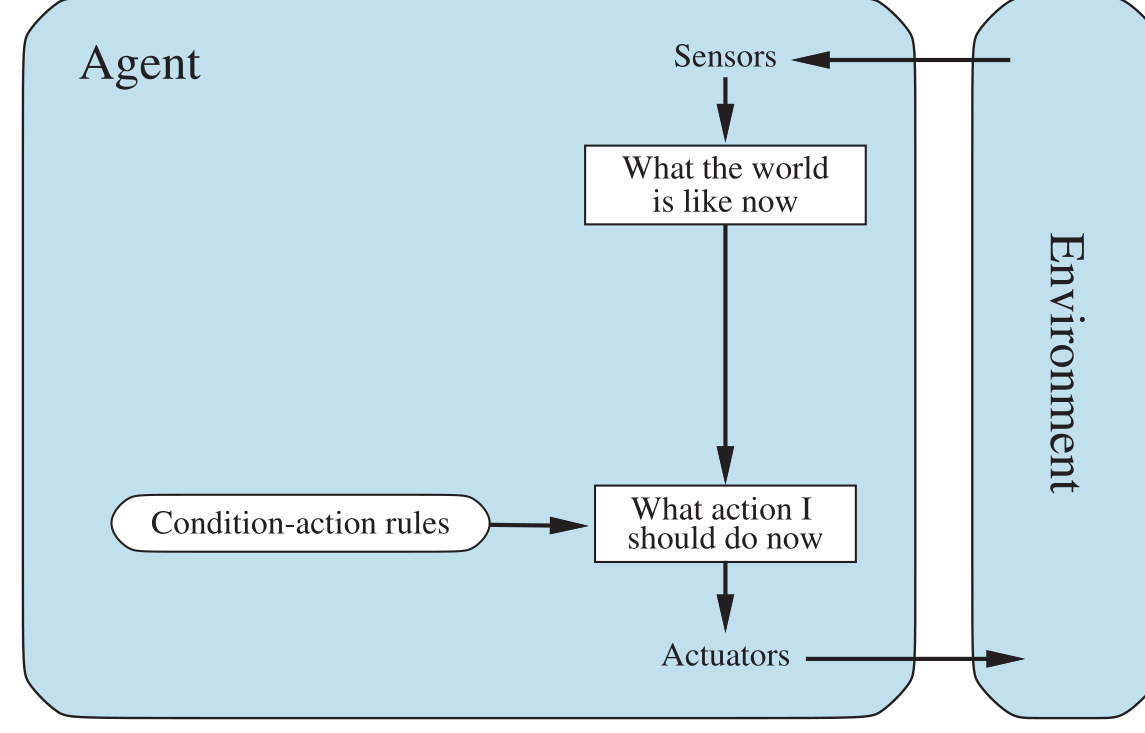
\includegraphics[width=\linewidth]{figures/aima-fig2-9.png}\\[-2pt]
    {\small (a) Simple reflex agent, Figure~2.9}
  \end{minipage}\hfill
  \begin{minipage}[t]{0.48\linewidth}\centering
    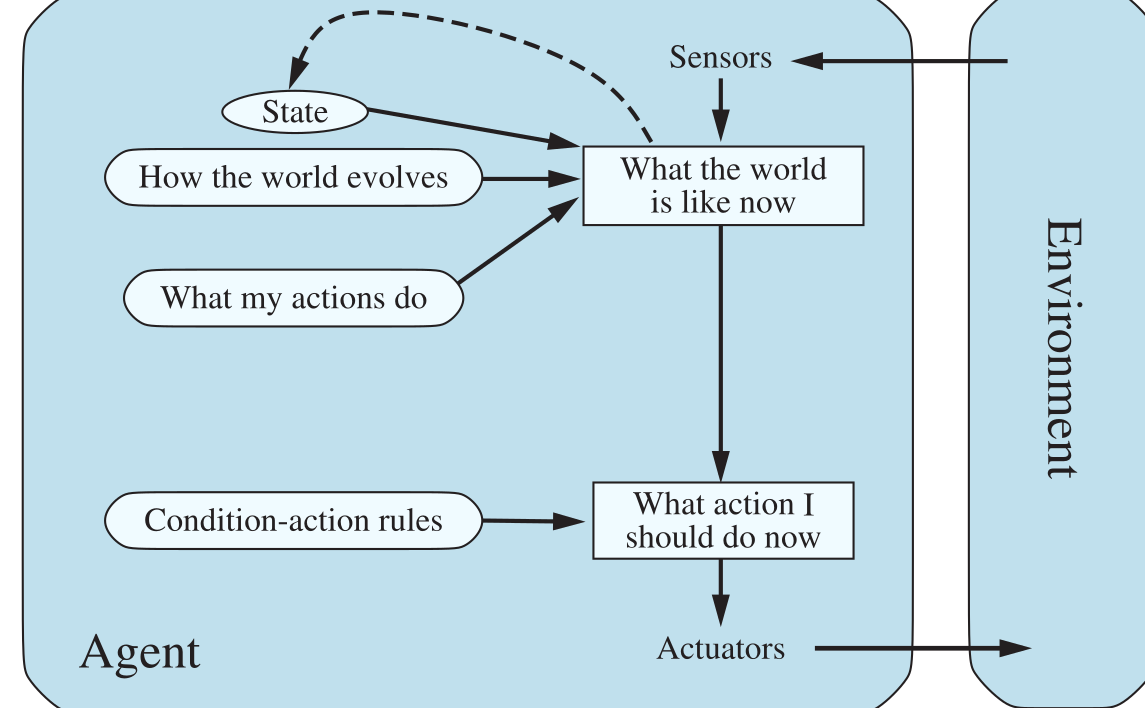
\includegraphics[width=\linewidth]{figures/aima-fig2-11.png}\\[-2pt]
    {\small (b) Model-based reflex agent, Figure~2.11}
  \end{minipage}\\[8pt]
  \begin{minipage}[t]{0.48\linewidth}\centering
    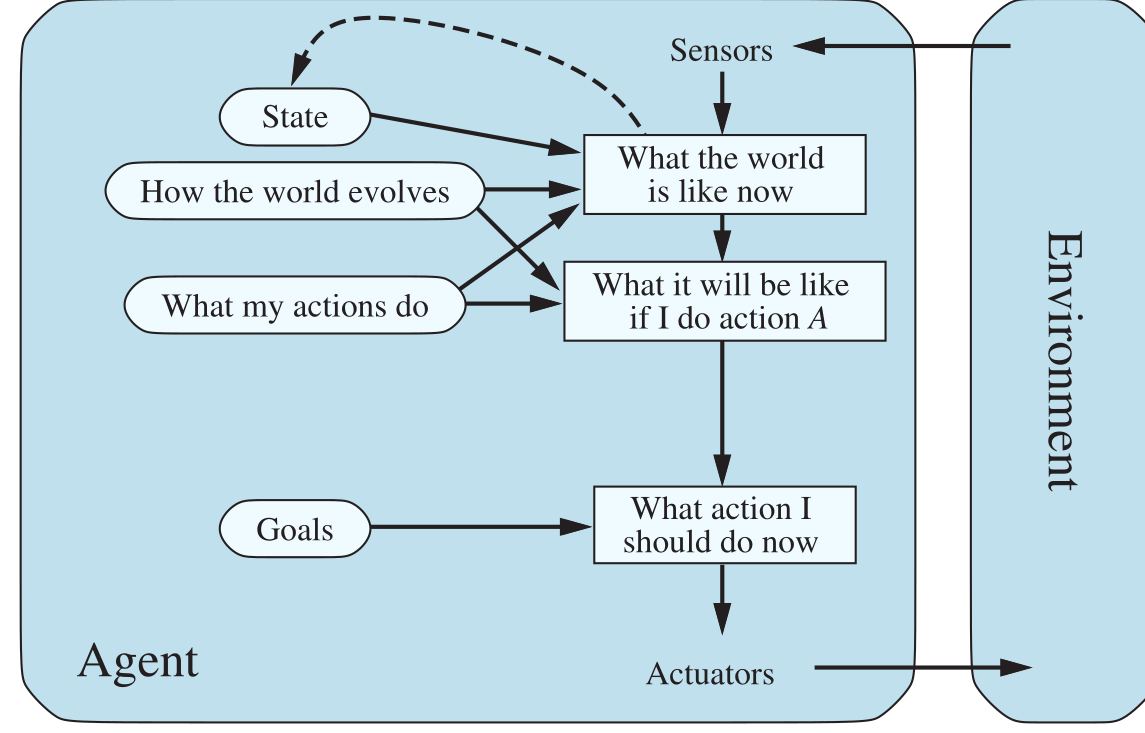
\includegraphics[width=\linewidth]{figures/aima-fig2-13.png}\\[-2pt]
    {\small (c) Model-based, goal-based agent, Figure~2.13}
  \end{minipage}\hfill
  \begin{minipage}[t]{0.48\linewidth}\centering
    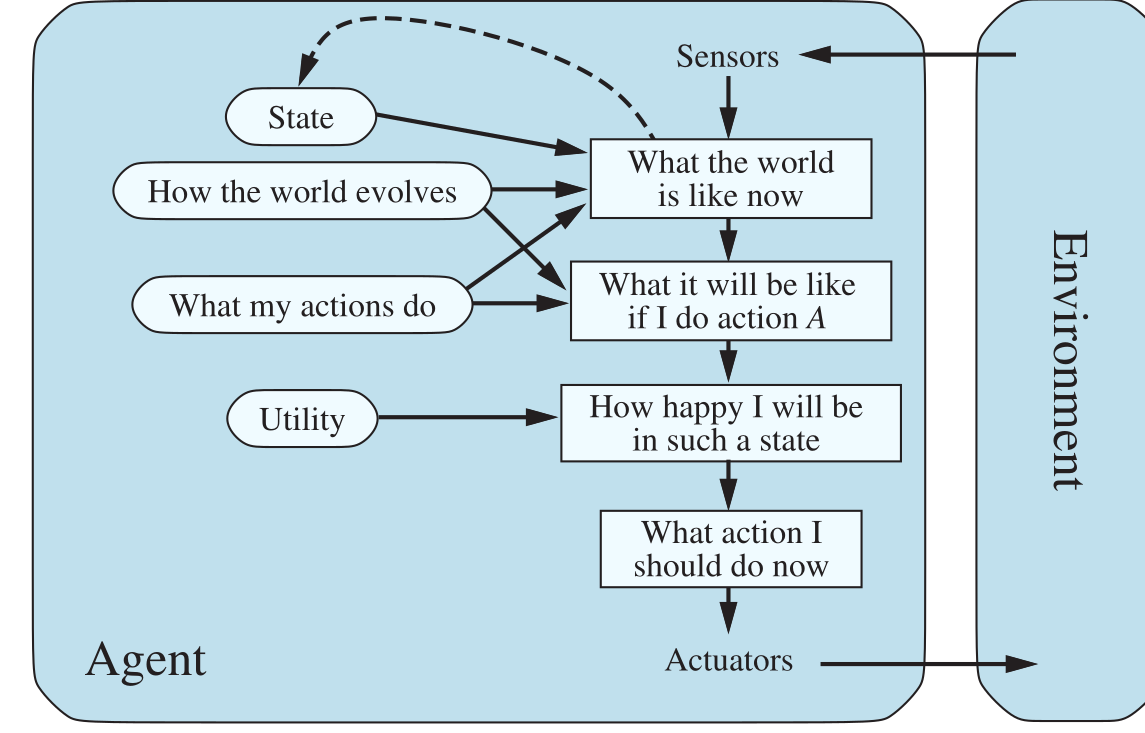
\includegraphics[width=\linewidth]{figures/aima-fig2-14.png}\\[-2pt]
    {\small (d) Model-based, utility-based agent, Figure~2.14}
  \end{minipage}
  \caption{The four agent programs, each adding one box to the one before: internal state with
  two models, then goals, then a utility. Figures~2.9, 2.11, 2.13, and 2.14 of
  \citet{russell2020aima}, reproduced from the Global Edition (\copyright~Pearson Education
  Limited 2022). Rectangles are the current internal state of the decision process; ovals are
  the background knowledge the process uses.}
  \label{fig:agents-programs}
\end{figure}

\subsubsection{Where the agents of this block fall}
\label{sec:agents-placement}

\paragraph{ReAct.}
ReAct augments ``the agent's action space to $\hat{A} = A \cup L$, where $L$ is the space of language''; a thought, an action in $L$, ``does not affect the external environment, thus leading to no observation feedback,'' and instead updates the context, $c_{t+1} = (c_t, \hat{a}_t)$, ``to support future reasoning or acting'' \citep[\S2]{yao2023react}.
The internal state of a ReAct agent is therefore its context: the trajectory of thoughts,
actions, and observations, with the task at its head. A frozen language model, prompted with
that context, computes the next action. In AIMA's terms this is a model-based agent whose state
is the trajectory and whose condition--action mapping is the language model. The goal sits in
the context, but there is no explicit plan and no explicit transition model, so it is not
goal-based in the strict sense. It is not a simple reflex agent, because its decision depends on
the whole trajectory and not on the current observation alone. ``Model-based'' here means the
state and the two models of the environment, not the language model inside.

\paragraph{Reflexion.}
Reflexion has ``three distinct models: an Actor, denoted as $M_a$, which generates text and actions; an Evaluator model, represented by $M_e$, that scores the outputs produced by $M_a$; and a Self-Reflection model, denoted as $M_{sr}$, which generates verbal reinforcement cues to assist the Actor in self-improvement'' \citep[\S3]{shinn2023reflexion}.
The actor is a ReAct or chain-of-thought agent; the evaluator scores a trajectory by exact match,
by a task-specific heuristic, or by another language model; the self-reflection output is stored
in memory and given to the next trial. This is the structure of AIMA's learning agent
(Figure~2.15 of AIMA): the actor is the performance element, the evaluator is the
critic, and the self-reflection model is the learning element. What it learns is text in the
next trial's context, not a change to the model's weights, and there is no problem generator.
The critic's standard, tests or exact match, is fixed outside the agent, which is what a critic
requires.

\paragraph{The patterns in Google's guide.}
Google's design-pattern guide sorts its patterns by orchestration \citep{google2026patterns}.
Under ``workflows that are deterministic'' it lists the sequential, parallel, and loop patterns, which run agents ``in a predefined, linear order'' on ``predefined logic without having to consult an AI model for the orchestration.''
Under ``workflows that require dynamic orchestration'' it lists the single-agent pattern, which ``uses an AI model, a defined set of tools, and a comprehensive system prompt,'' the coordinator and hierarchical patterns, in which a model decides which agent runs next, the review-and-critique and iterative-refinement patterns, and ReAct itself.
In AIMA's terms the single agent is ReAct's structure. A deterministic workflow is a program
whose control decisions are all made at design time, with the model filling in content. The
coordinator and hierarchical patterns move one more decision, which agent runs next, to run
time. Review-and-critique and iterative refinement add a critic and an attempt loop, the
learning agent's structure without a change to weights. None of the patterns computes expected
utility; cost is bounded by the runtime, not weighed by the agent. \Cref{sec:patterns} takes the
guide up on its own terms.

\paragraph{\msa{}.}
The five versions walk the same structures in order, on one task. V0 is a fixed workflow: the
model fills in content and never chooses the next operation, and only the runtime's phase
boundary ends the run. V1 is ReAct's structure: the trajectory is the state and the model
chooses the next action from it. V2 is goal-based: an explicit plan in state, revised when a
planned step fails. V3 adds the critic: a validator that applies a fixed standard, the patch
applies, the tests the agent claims to have run did run, and the hunks touch lines that exist.
V4 is Reflexion's structure: the validator's rejection triggers a reflection whose text enters
the next attempt's context. No version learns weights, none has a problem generator, and none
computes expected utility; the budget is enforced by the runtime. \Cref{tab:agents-placement}
collects the placements.

\begin{table}[htbp]
  \caption{The agents of this block in AIMA's program structures. ReAct and Reflexion are the
  published systems; the guide's rows are its pattern families; V0 to V4 are our versions. The
  placements of the guide's patterns and of our versions are our reading.}
  \label{tab:agents-placement}
  \small
  \begin{tabularx}{\linewidth}{>{\RaggedRight}p{2.9cm}>{\RaggedRight}p{2.9cm}XX}
    \toprule
    Agent & AIMA structure & Internal state & Decided by a model at run time \\
    \midrule
    ReAct & Model-based & The trajectory (context) & The next action, including thoughts, and when to finish \\
    Reflexion & Learning agent: actor, critic, learning element & The trajectory; long-term reflection memory & The actor's actions; the reflection text; the critic's score when the evaluator is a model \\
    Guide: sequential, parallel, loop & Fixed workflow & Each agent's own context & Content only; the order is predefined logic \\
    Guide: single agent, ReAct & Model-based & The context & The next action and tool call \\
    Guide: coordinator, hierarchical & Model-based with model-chosen routing & The coordinator's context and the workers' results & Which agent runs next; how subgoals are assigned \\
    Guide: review-critique, iterative refinement & Learning agent's structure & The candidate and the critique & The candidate; the critique; whether to iterate \\
    V0 & Fixed workflow & The chain's fixed artifacts & Content only: the localized file, the lines, the patch text \\
    V1 & Model-based & The trajectory & The next action and when to submit \\
    V2 & Goal-based & The trajectory and an explicit plan & The plan; its revision when a step fails \\
    V3 & V2 plus a critic & As V2, plus the validator's decision & The candidate patch; the validator's semantic judgement \\
    V4 & Learning agent's structure & As V3, plus retained reflection guidance & The reflection text and the next plan; not whether another attempt is allowed, which the runtime decides \\
    \bottomrule
  \end{tabularx}
\end{table}

Moving down the structures buys adaptability and costs model-call overhead, because computing
more at run time means more calls to whatever does the computing. It costs inspectability,
because a rule that fired is easier to point at than a plan that was searched for. And it
changes failure propagation, because state carried forward carries errors forward; here an
edit carried forward carries a wrong edit into every later test run. Termination arises above only for the reflex agent. We must raise it for every program that
computes its next action at run time, since such a program can compute one forever, and the
runtime, not the program's decision logic, owns the stopping rule.

